\documentclass[conference]{IEEEtran}
\IEEEoverridecommandlockouts
% The preceding line is only needed to identify funding in the first footnote. If that is unneeded, please comment it out.
\usepackage{cite}
\usepackage{amsmath,amssymb,amsfonts}
\usepackage{algorithmic}
\usepackage{graphicx}
\usepackage{textcomp}
\usepackage{xcolor}
\def\BibTeX{{\rm B\kern-.05em{\sc i\kern-.025em b}\kern-.08em
    T\kern-.1667em\lower.7ex\hbox{E}\kern-.125emX}}
\begin{document}

\title{Segmentation and background detection for human identification\\
}

\author{\IEEEauthorblockN{1\textsuperscript{st} Mikel-ange Barros}
\IEEEauthorblockA{\textit{computer science department} \\
\textit{University Claude Bernard Lyon 1}\\
Lyon, France\\
mikel-ange.barros@etu.univ-lyon1.fr}
\and
\IEEEauthorblockN{2\textsuperscript{nd} Zacharia Beddalia}
\IEEEauthorblockA{\textit{computer science department} \\
\textit{University Claude Bernard Lyon 1}\\
Lyon, France \\
zacharia.beddalia@etu.univ-lyon1.fr}
}

\maketitle

\begin{abstract}
Image processing is a set of fundamental researc in areas of image pattern based recognition.
In this research, segmentation methods are the core to analyze a given image.
This document present our method of segmentation and how it is used to detect moving bodies in a video.
We will show our method by explaining the algorithms and their implementations, and we will compare it to other existing method.
\end{abstract}

\begin{IEEEkeywords}
segmentation, body detection
\end{IEEEkeywords}

\section{Introduction}
Image analysis is a branch of computer science with an increasing number of different applications, whether in the field of video games, medicine or data protection. All of these technologies use an image segmentation method, setting up adapted segmentation methods to these different applications is therefore an important part of the researches to be carried out. Our work is moving in this direction in order to obtain convincing results in the detection of human bodies in motion.

\section{Image Segmentation}

Image segmentation is the first stage of processing an image. For the segmentation to be deemed effective, many criteria must be met. Among these criteria, we can notably note the speed of the execution as well as the precision of the detected zones. As said, Image Segmentation is an important field of image analysis and for a better comprehension of it, image segmentation is split in four different methods :

\begin{itemize}
\item Segmentation by edges detection : this type of segmentation tries to detect the contours of different objects in order to identify them. In this type of segementation, we can find the usage of Canny's edges detections.
\item Segmentation by thresholding : This type of segmentation detects the colour of differents objects in order to identify them. With this technique, we will try to separate an object in a color spectrum compared the rest of the objects. In this type of segementation, we can notice adaptive thresholding techniques.
\item Segmentation using Feature Based Clustering : cluster composed of pixels with the same characteristics are detected to define shapes. The differences between this method and the region based one is that a cluster is not necessarily composed of adjacent pixels, unlike a region. K-means algorithm is an implementation of this method.
\item Segmentation region based: This type of segmentation tries to determine regions composed of pixels with the same caracteristics. 
\end{itemize}

In this paper, the methods used is a single seeded region growing. We will compare it to the K-means Algorithm and the watershed algorithm implementation of the library OpenCV.

\subsection{Single Seeded Region Growing}

This segmentation method is based on the selection of random pixels, called seed. Thus, during the execution of this algorithm, a certain number of pixels will be selected in order to serve as a center for our region. Once these points have been selected, the algorithm will make the regions grow by processing the pixels directly close to it. A pixel with a similar caracteristic, usually its color or intensity, is added to the region and removed from the list of available pixels. At the end of this phase, the algorithm has produced one region per seed that must be merged together if they are similar enough, that again, based on a caracteristic given to the algorithm.

This algorithm is usually applied to a grayscale image.


\subsection{OpenCV K-means algorithm}

In order to be able to execute this algorithm, we must first define the number of clusters with which the image will be cut out. After this has been done, the algorithm will place points, called the center of the cluster, and will add the pixels of the image to the clusters while trying to minimize a function.

This algorithm is usually applied to a color image.

\subsection{OpenCV watershed algorithm}

Each grayscale image can be seen as a heightmap, where high intensity value denotes peaks and low intensity value denotes valleys. The algorithm uses the peaks and valley to determine the position of local minimal value and start filling each basins with different colored water (labels). As the water rises, depending on the peaks nearby, water from different basins, obviously with different colors will start to merge. However, we do not want all regions to merge.
For this, OpenCV implements an algorithm where it has defined in advance where will be the zones which can merge, and which cannot. For this, we use first a segmentation by edge detection.

This algorithm is usually applied to a grayscale image.

\section{Our Algorithm}

\subsection{Basic principle}

As told above, our algorithm is based on the principle of a single seeded region growing. As defined above, we will therefore randomly place seed on the given image. These points will serve as base for the rest of the algorithm. The main difference between our algorithm and a classic single seeded region growing segmentation is that our algorithm is applied to a color image. 

\subsection{Data structure}

To implement this algorithm we need a data structure to store the useful information. As our algorithm is based on a region-based algorithm, it seemed logical to use a data structure to represent a region. Thus, we define each zone of our segmented images as being a structure containing :
\begin{itemize}
\item a list of the pixels of the region : this is our way to determine which pixel belong to which region.
\item a list of its neighbours : for the region merging part of the algorithm, we need to keep updated and adjacency list for each region.
\item a list of its borders : for the purpose of displaying it without having to calcul it on an already segmented image.
\item the average color of the pixels belonging to the region : here again, for the region merging part of the algorithm.
\end{itemize}
Thanks to this structure we can easily interact on our region, create and modify them which will serve us for the future, the region growing.

\subsection{Region growing}

In order to start our region growing, we need to define the points. Those point represent a pixel of the image, from which our regions will start to grow. For this, we randomly select a number of points. This number is given as a parameter of the algorithm. We proceed to create as many regions as there are points. We then assign each point to a region and this point will serve as the starting point for the enlargement of our regions. In order to define that a point in a region has already been processed, each of the points already visited is kept and marked as visited : we do not want to process a point more than once.
Once this has been defined, we can move on to the main loop of our region growing and loop over each regions and at each iteration for a pixel in the region, we look at the 8 neighboring pixels. For every adjacent pixel of the current one, we verify: 
\begin{itemize}
\item If this pixel already belong to the current region, we continue. 
\item If this pixel is not marked by another region, then we calculate the euclidian distance between the color of the pixel belonging to the region and the color of the processed pixel. If the color of the pixel is at a distance below a user-defined threshold, then it is added to the region, otherwise it is added to the border of the region.
\item If this pixel is already marked by another region, we add this region to the list of neighbours of the current pixel region. If the distance betweend the two pixel is greater than the other threshold used in the region merging part of the algorithm (see after), then the processed pixel is flagged as a border pixel.
\end{itemize}

This part of the algorithm stops when all the marked pixels have been processed. 

At the end of our region growing , we calculate the average color of each region's pixels to use it for the merging of the regions.


\subsection{Region merging}

In this part of our code, we will merge all similar and neighbouring regions. To reach that, we will use a Region Adjacency Graph (RAG) using the adjacency list of each region that were filled in the previous step of the algorithm. We look for each region neighbours to see if they have a similar average color. We then calculate the euclidean distance between the two averages and see if it is below a second threshold. If the two regions have similar enough colors, we merge them. A region is not litteraly merged but instead it is eaten :
the region that has eaten it has now its neighbour, all of its neighbour adjacency lists are updated accordingly and the region is deleted. We recalculate the value of the average color of the bigger region.

When all the regions have been processed, we finish the execution and display the segmented image.


\subsection{Comparative result}

As explained above, we compare the results obtained by our algorithm to the results of a k-means algorithm and to those of a watershed algorithm. First, we can see that the different zones are fairly well recognized by our algorithm (b) and the k-means algorithm (c). We can also notice that the watershed  (d) does not seem to adapt to the analysis of an image of this type. We will therefore exclude this algorithm for the following steps.
Now looking at the last two algorithms, we can notice that the k-means produces regions which limit are less clean and smooth than with our algorithm. Despite the fact that the k-means algorithm makes it possible to segment the image in more detail, our algorithm makes it possible to identify the general shapes of objects with more precision, which is more suitable for detecting human bodies in the original image (a). 

\begin{figure}[h!]
  \centering
  \begin{tabular}{@{}c@{}}
    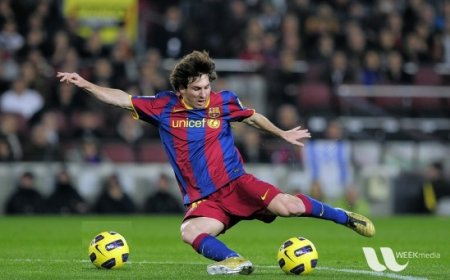
\includegraphics[width=0.4\linewidth]{fig0.jpg} \\[\abovecaptionskip]
    \small (a) basic image
  \end{tabular}
  \begin{tabular}{@{}c@{}}
    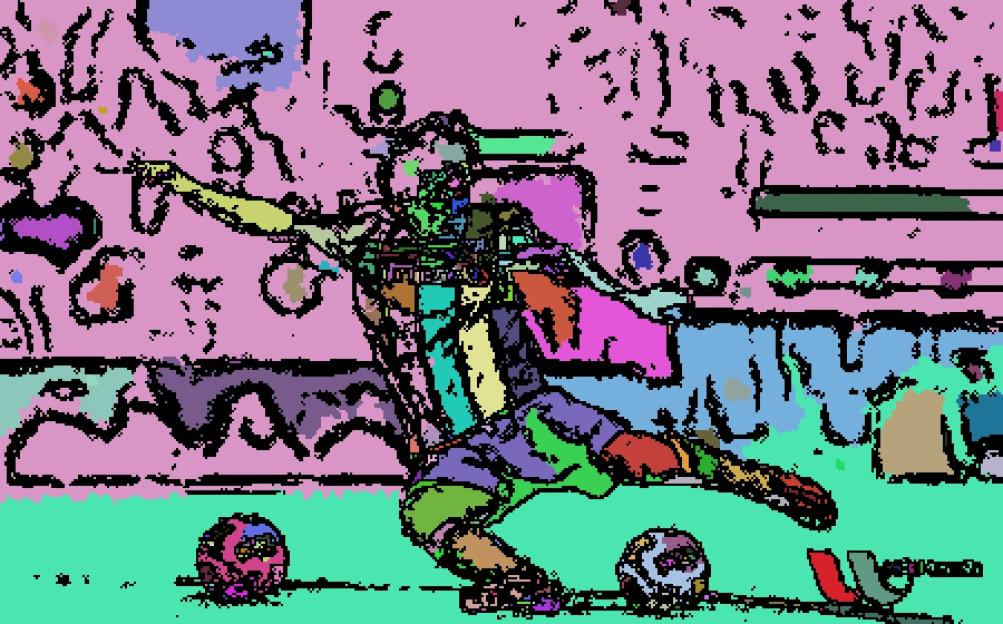
\includegraphics[width=0.4\linewidth]{fig1.jpg} \\[\abovecaptionskip]
    \small (b) our result
  \end{tabular}

  \vspace{\floatsep}

  \begin{tabular}{@{}c@{}}
    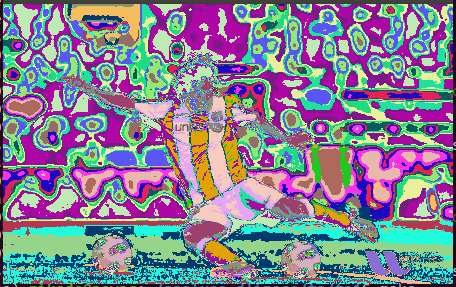
\includegraphics[width=0.4\linewidth]{fig2.png} \\[\abovecaptionskip]
    \small (c) k means result : 32 cluster
  \end{tabular}
  \begin{tabular}{@{}c@{}}
    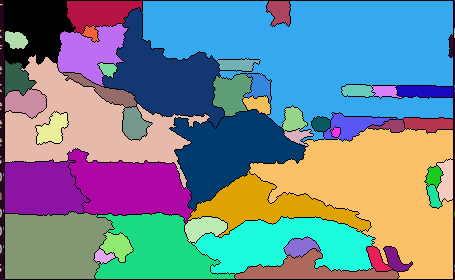
\includegraphics[width=0.4\linewidth]{fig3.png} \\[\abovecaptionskip]
    \small (d) watershed result
  \end{tabular}
  \caption{comparative results}
  \label{fig 1}
  
\end{figure}

\subsection{Limit of our algorithm}

Our implementation possesses three identifiable problems:

Firstly, if two different elements have a similar color they will be considered identical when they should not.
Secondly, during the growing of the region, if a pixel has not been reached, then it will not belong to any region. However if the amount of seed is high enough, this will only concern a very few number of scatered pixels on highly detailed images, which doesn't affect the segmentation.
Finally, our algorithm is highly dependent on the parameters passed by the user. Indeed, whether it is the number of seeds to be placed or the value of the thresholds, everything must be defined by the user. And depending on the choices made by the latter, the results obtained can be very different (fig 2).

\begin{figure}[h!]
  \centering
  \begin{tabular}{@{}c@{}}
    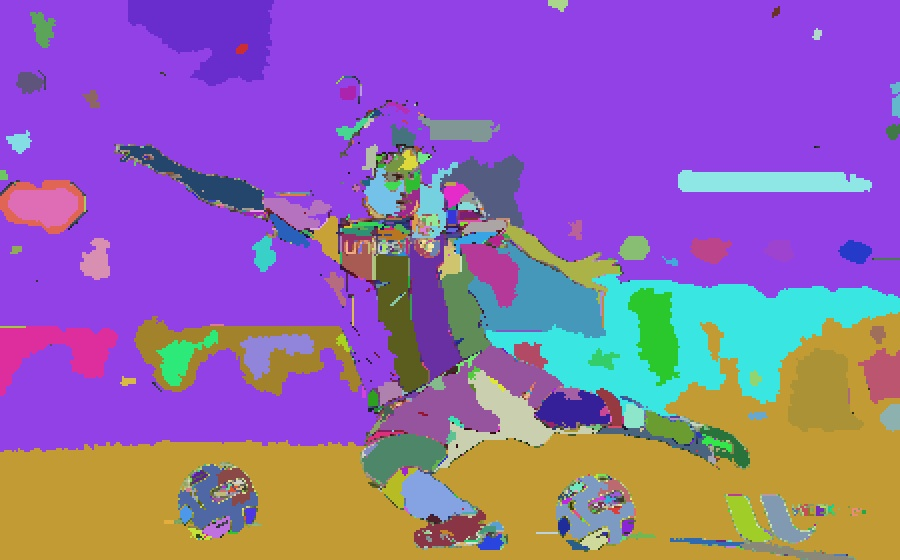
\includegraphics[width=0.4\linewidth]{fig7.jpg} \\[\abovecaptionskip]
    \small (a) Result with hight threshold
  \end{tabular}
  \begin{tabular}{@{}c@{}}
    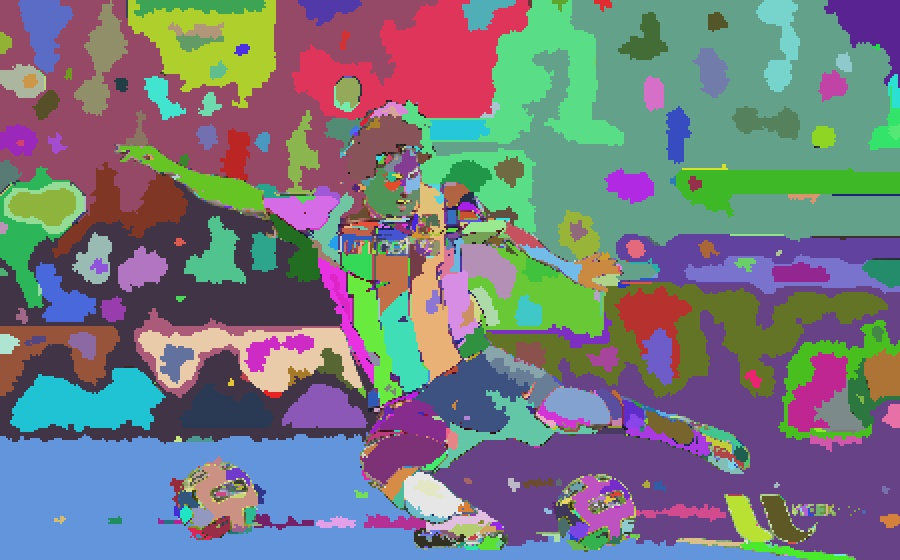
\includegraphics[width=0.4\linewidth]{fig8.jpg} \\[\abovecaptionskip]
    \small (b) Result with medium  threshold
  \end{tabular}

  \vspace{\floatsep}

  \begin{tabular}{@{}c@{}}
    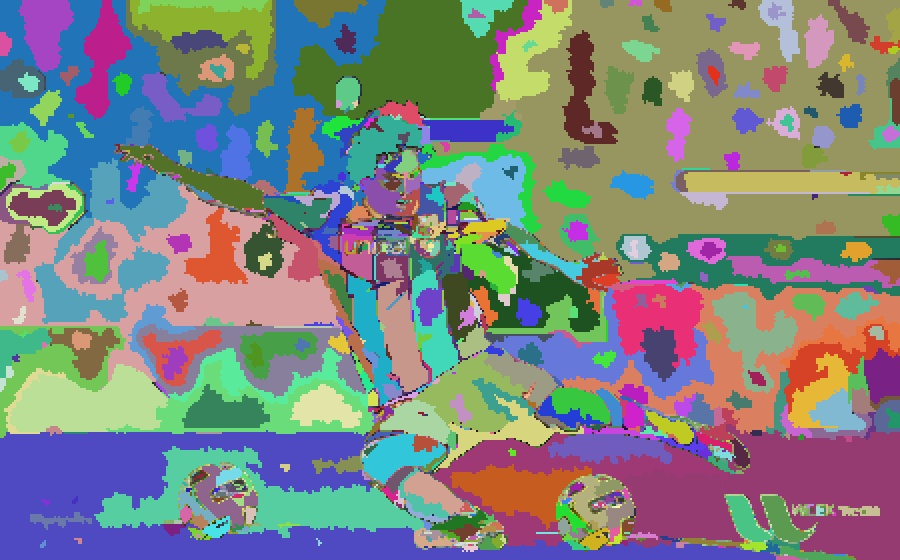
\includegraphics[width=0.7\linewidth]{fig9.jpg} \\[\abovecaptionskip]
    \small (c) Result with low threshold
  \end{tabular}
  \caption{result of our algorithm with different settings}
  \label{fig 2}
  
\end{figure}


\section{Foreground Detection}

In order to allow Foreground detection on videos, OpenCV provides two tools, the first being the background detector and the second being the motion detection. After different tests, it seemed to us that the results outputed by the two classes were very similar and as the movement detection was faster at execution we decided to use it.

\subsection{Movement detection}
 
The OpenCV movement class implement two method to analyse the movement, the Lucas-Kanade algorithm and the Farneback’s algorithm, which is an extending of the Lucas-Kanade. The Farneback’s algorithm seems to be the most suitable for character detection because it allows to surround the moving area. Before proceeding with an analysis of the movement, we must first eliminate the noise, preventing the risks of it being identified as a moving part on the video. For this, we use the OpenCV function: fastNlMeansDenoisingColored which will remove the noise on a colored image, genereted by the video encoding mostly.
With this allgorithm, we manage to identify the moving elements and cut out the background elements, from the basic image (a), unusable as is, for our body detection.
After this movement detection, we obtain a result (b) with the body shapes cropped from the background.

\begin{figure}[h!]
  \centering
  \begin{tabular}{@{}c@{}}
    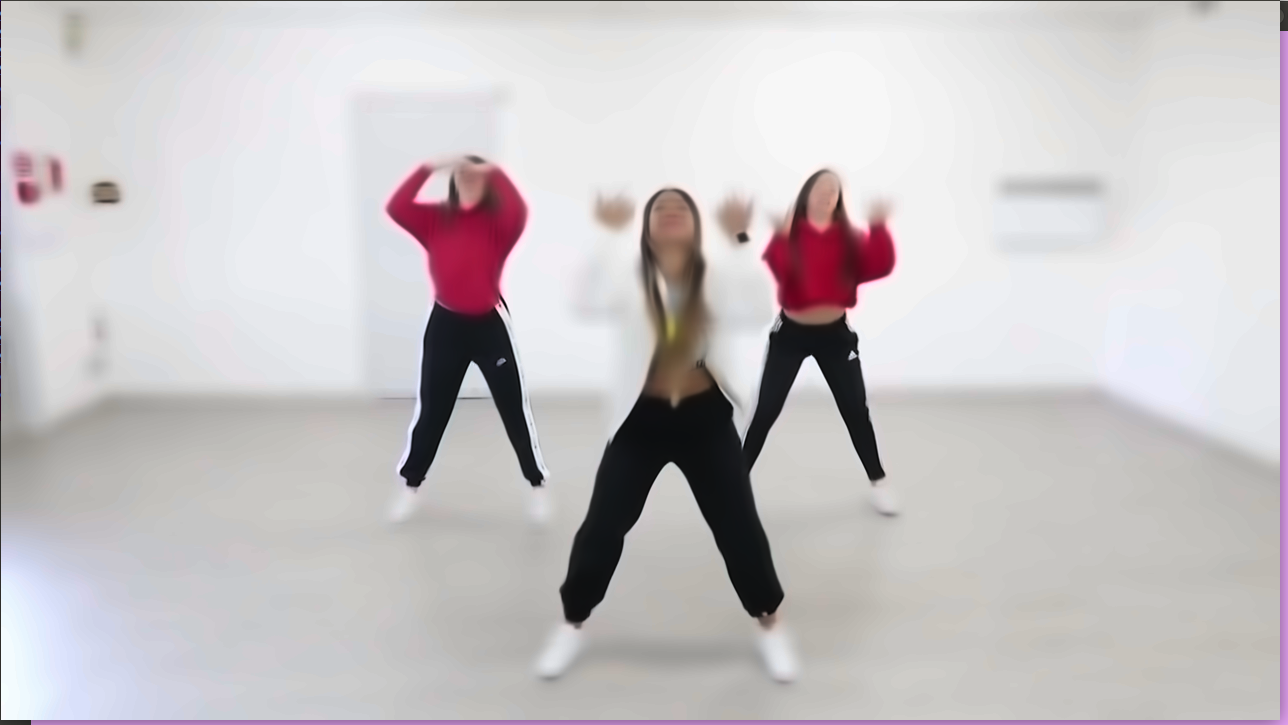
\includegraphics[width=0.4\linewidth]{fig5.png} \\[\abovecaptionskip]
    \small (a) basic image
  \end{tabular}
  \begin{tabular}{@{}c@{}}
    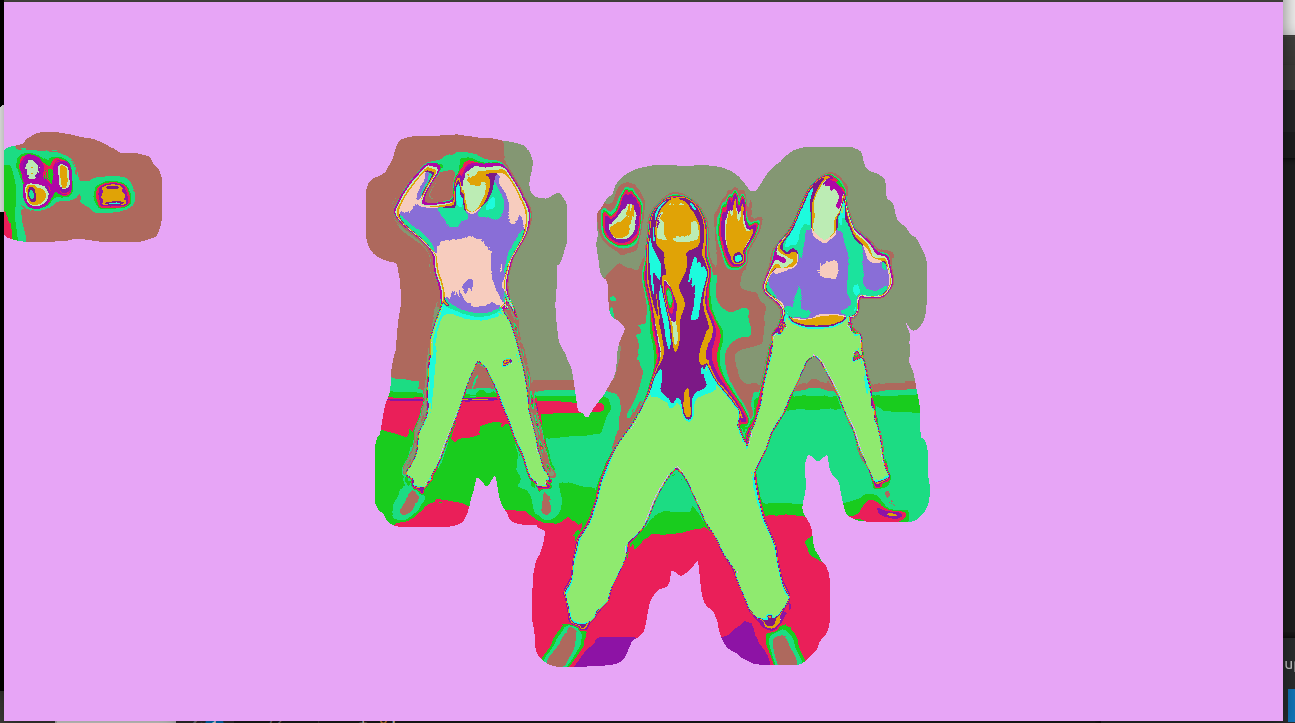
\includegraphics[width=0.4\linewidth]{fig6.png} \\[\abovecaptionskip]
    \small (b) movement detection result
  \end{tabular}
  \caption{Movement detection}
  \label{fig 3}
\end{figure}

\subsection{Segmentation and body detection}

Once we have been able to detect the movements on our image, we must now look into a more precise analysis of the elements. Indeed, as you can see, part of the background is cut with the people we want to detect. This is where our segmentation becomes useful. We use the defined zones to determine which ones are really moving and which are not. For this, we compare for each area the number of pixels in the area and the number of moving pixels in the area. If more than 50 percent of the pixels in the area are in motion, we consider that all region is actually in motion and we cut it out. Otherwise we consider it to be background and we do not cut it. 

This method, gives us good results (fig 4).

\begin{figure}[h!]
  \centering
  \begin{tabular}{@{}c@{}}
    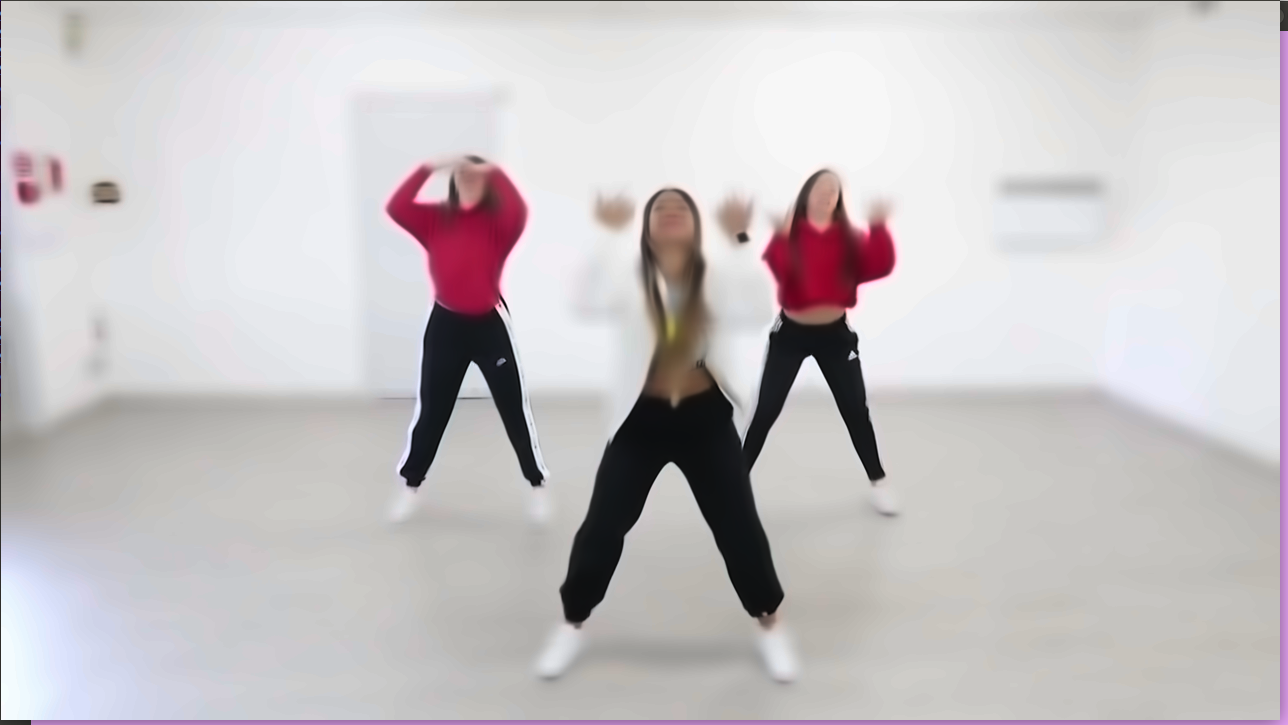
\includegraphics[width=0.4\linewidth]{fig5.png} \\[\abovecaptionskip]
    \small (a) basic image
  \end{tabular}
  \begin{tabular}{@{}c@{}}
    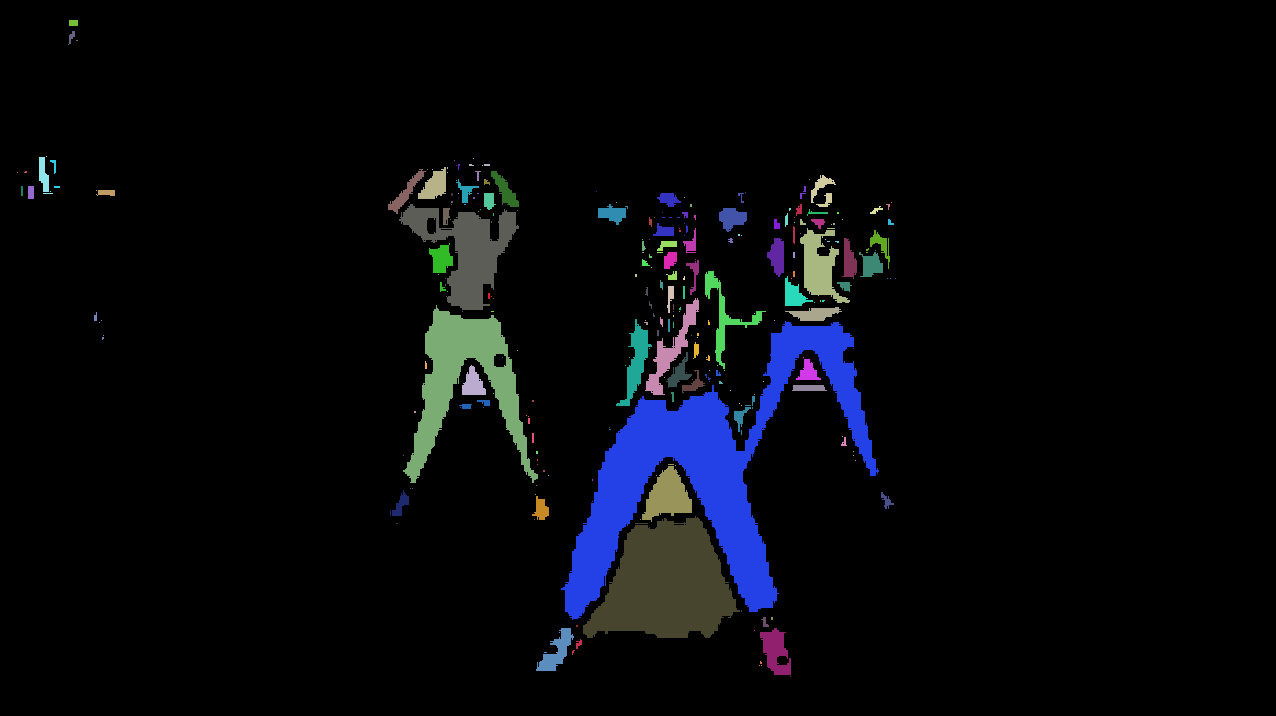
\includegraphics[width=0.4\linewidth]{fig10.png} \\[\abovecaptionskip]
    \small (b) foreground segmentation result
  \end{tabular}
  \caption{Movement detection}
  \label{fig 3}
\end{figure}

\section{Conclusion}

To conclude, this project allowed us to enter the field of image analysis and to discover the importance of segmentation within numerous analysis methods. Moreover, this allowed us to develop our own method of segmentation and to apply it in a specific area, the analysis of the human body. The method implemented returns rather satisfying results allowing us to imagine a place for our segmentation algorithm in the detection of human body on a video.


\section*{Acknowledgment}

Thanks to Ms. Saida for this project, her help and mostly for her understanding of the particular situation during which this study was made.

\section*{References}

\vspace{12pt}
\color{red}

\end{document}
